\documentclass[12pt,a4paper]{report}
\usepackage[italian]{babel}
\usepackage{newlfont}
\usepackage{color}
\textwidth=450pt\oddsidemargin=0pt

\usepackage[utf8x]{inputenc}
\usepackage{graphicx}
\usepackage{amsmath}
\usepackage{amssymb}
\usepackage{setspace}

\begin{document}

% qui comincia il titolo
\begin{titlepage}
\begin{center}
{\Large{\textsc{Università degli studi di Roma $\cdot$ Tor Vergata}}} 
\rule[0.1cm]{15.8cm}{0.1mm}
\rule[0.5cm]{15.8cm}{0.6mm}
\\\vspace{3mm}

{\small{\bf Macroarea di Lettere e Filosofia \\ Master in Sonic Arts}}

\end{center}

\vspace{23mm}

\begin{center}
\begin{spacing}{1.7}
\textcolor{black}{
\linespread{5}
{\LARGE{\bf 
TITOLO
}}}

\end{spacing}
\end{center}

\vspace{50mm} \par \noindent

\begin{minipage}[t]{0.47\textwidth}

{\large{\bf Relatore: \vspace{2mm}\\\textcolor{black}{
Prof. Giuseppe Silvi}\\\\

%\textcolor{red}{
%\bf Correlatore: (eventuale)
%\vspace{2mm}\\
%Prof./Dott. Nome Cognome\\\\}
}
}
\end{minipage}
%
\hfill
%
\begin{minipage}[t]{0.47\textwidth}\raggedleft \textcolor{black}{
{\large{\bf Presentata da:
\vspace{2mm}\\
%
% INSERIRE IL NOME DEL CANDIDATO
%
Lorenzo Ferri}}}
\end{minipage}

\vspace{17mm}

\begin{center}

{\large{%\bf Sessione \textcolor{black}{ I }
%\vspace{2mm}\\

Anno Accademico \textcolor{black}{2016/17}}}
\end{center}

\newpage\null\thispagestyle{empty}

\end{titlepage}
% qui finisce il titolo

\tableofcontents

\listoffigures


\addcontentsline{toc}{chapter}{Elenco delle figure}

\chapter*{Abstract}

Nel corso di questa tesi si cercherà di rispondere ad una semplice domanda: posso svincolarmi dal fatto che un format audio possa essere riprodotto solo dalla configurazione di riproduzione adatta?\\

La risposta è si, in quanto esistono già tecniche che trasformano un format in un altro adatto ad un'altra configurazione ma, cercherò di introdurre, nella prima parte di questa tesi, un \textbf{format} "generale" che non ha bisogno di dover passare da questo stadio di trasformazione (in quanto esso stesso non è inizialmente adattato per nessuna configurazione di riproduzione), sto parlando del format \textbf{Multi-Dimesional Audio MDA} orientato verso l'\textbf{audio ad oggetti} (object-oriented).\\

In una seconda parte invece cercherò di implementare l'MDA in alcune delle più comuni configurazioni di riproduzione servendomi della tecnica di spazializzazione \textbf{Vector-Base Amplitude Panning VBAP} di cui spiegherò anche il funzionamento.\\

Infine farò degli esempi adattando il format MDA nelle configurazioni quadrifonica, 5.1 e stereo.
\addcontentsline{toc}{chapter}{Abstract}


\chapter{Dai canali audio agli oggetti sonori}

Siamo all'inizio di questa tesi, l'abstract ci ha permesso di capire qual'è il nostro scopo e i passaggi che percorrerà questa stesura, ora non rimane che cominciare.\\

Nel mondo odierno l'avanzamento tecnologico ha permesso a tutti coloro che ne hanno voglia la possibilità di poter ascoltare un contenuto sonoro, basti pensare a chi ha un hi-fi in casa, chi un impianto per home-theater o chi direttamente va al cinema; in tutte queste situazioni l'ascoltatore ha accesso a questi contenuti diciamo in modo "smart" cioè senza preoccuparsi di tutto il lavoro e la progettazione che sta dietro alla realizzazione del contenuto e sulla sua successiva riproduzione, questo è possibile grazie a delle "regole" che stanno alla base di tutta questa catena; un esempio chiarirà meglio l'uso improprio della parola regola.\\

Consideriamo per esempio un cinema, sappiamo dall'acustica che il modo in cui sono progettati i diffusori e la sala di proiezione coloreranno \footnote{con il termine colorare nell'audio e in acustica si intende la tendenza di un sistema a modificare lo spettro in frequenza di un segnale audio che vive al suo interno} in qualche maniera il suono e quindi non faranno ascoltare lo stesso contenuto che è stato creato per quel film, è quindi d'obbligo per il cinema (almeno lo spero) tarare l'ascolto in modo che non ci sia questa colorazione, qui per esempio il fatto di rendere lineare il suono costituisce una regola, uno standard che è necessario affinché si abbia un giusto ascolto del contenuto.\\

Come quest'ultima ci sono diverse regole, diversi standard da rispettare per garantire che il produttore di contenuti sonori e l'ascoltatore abbiano accesso alla stessa informazione, nel nostro caso siccome la tesi è mirata ad un solo aspetto dell'audio, faremo riferimento solo a quelle regole che stanno a base della spazializzazione sonora, quindi quegli standard che hanno a che fare in qualche modo con la geometria di riproduzione.\\

Ora è d'obbligo fermarsi un attimo e ripercorrere brevemente alcuni degli standard in modo da capire in che punto vogliamo intraprendere una strada concettualmente diversa, anche perchè alla fine del ragionamento dovremo ricollegarci ad essi.


\section{Standard di riproduzione}\label{metodi}

\subsection{Audio in una dimensione}

Il primo metodo descritto (e forse il più importante) è lo \textbf{STEREO}\footnote{qui c'è da fare una precisazione utilizzato la parola stereo, perchè e comune utilizzarlo in casistiche sbagliate in quanto, formalmente, lo stereo è una modalità di riproduzione e di registrazione che oltre ad usare la IID utilizza anche la ITD ed è come se i due canali di questo standard conterrebbero esattamente quello che sentirebbero le nostre orecchie}(configurazione 2.0) in cui avendo a disposizione due speaker la sensazione di spazialità viene data dalla differenza di potenza del segnale inviati agli speaker, infatti se il segnale risulta più forte in uno dei due, la sorgente fantasma risulterà più spostata verso quest'ultimo.\\

\begin{figure}[htbp]
	\centering
	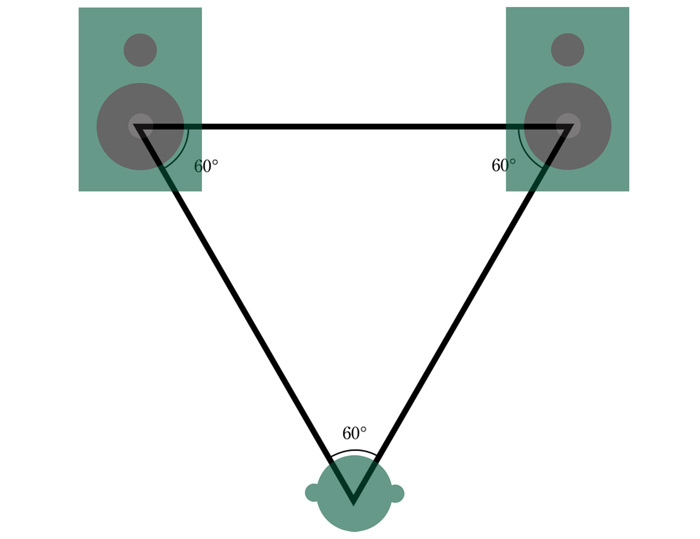
\includegraphics[scale=0.30]{figures/stereo.jpg}
	\caption {Configurazione stereo} 
	\label{fig:stereo}
	\end{figure}

Parlando dello stereo cominciamo a parlare di standard in quanto la configurazione prevede di creare un triangolo equilatero con ai vertici i due altoparlanti e l'ascoltatore,  quindi se non si segue il collocamento delle casse a $\pm 30°$ non si avrà la giusta spazialità e collocazione dei suoni.\\

L'ascolto di musica si ferma generalmente qui ma l'avvento dei film e dei cinema ha portato al concetto di audio in due dimensioni in particolare al surround.

\subsection{Audio in due dimensioni}

Per audio in due dimensioni si intende una riproduzione che pone l'ascoltatore al centro di un piano di diffusione in modo che si possano sentire suoni provenienti anche dai lati e da dietro; diverse sono le configurazioni possibili ma quelle che interessano a noi sono principalmente tre.\\

La più diffusa configurazione surround è sicuramente la \textbf{5.1} \footnote{dove la prima cifra sta per il numero di diffusori nel piano e la seconda cifra sta per il numero di LFE (canale audio dedicato agli effetti a a bassa frequenza)} usata principalmente dalla Dolby e dalla DTS per riproduzione di audio per film.


Questa configurazione, come spiega da specifica \cite{5.1}, è composta da un canale LFE per il subwoofer e di 5 canali distribuiti in 5 satelliti disposti rispettivamente a 0°, $\pm30°$ e $\pm110/120°$\\

Una successiva configurazione è la \textbf{7.1} che riporta angoli di 0°, $\pm30°$, $\pm90/110°$ e $\pm135/150°$\\

\begin{figure}[htbp]
	\centering
	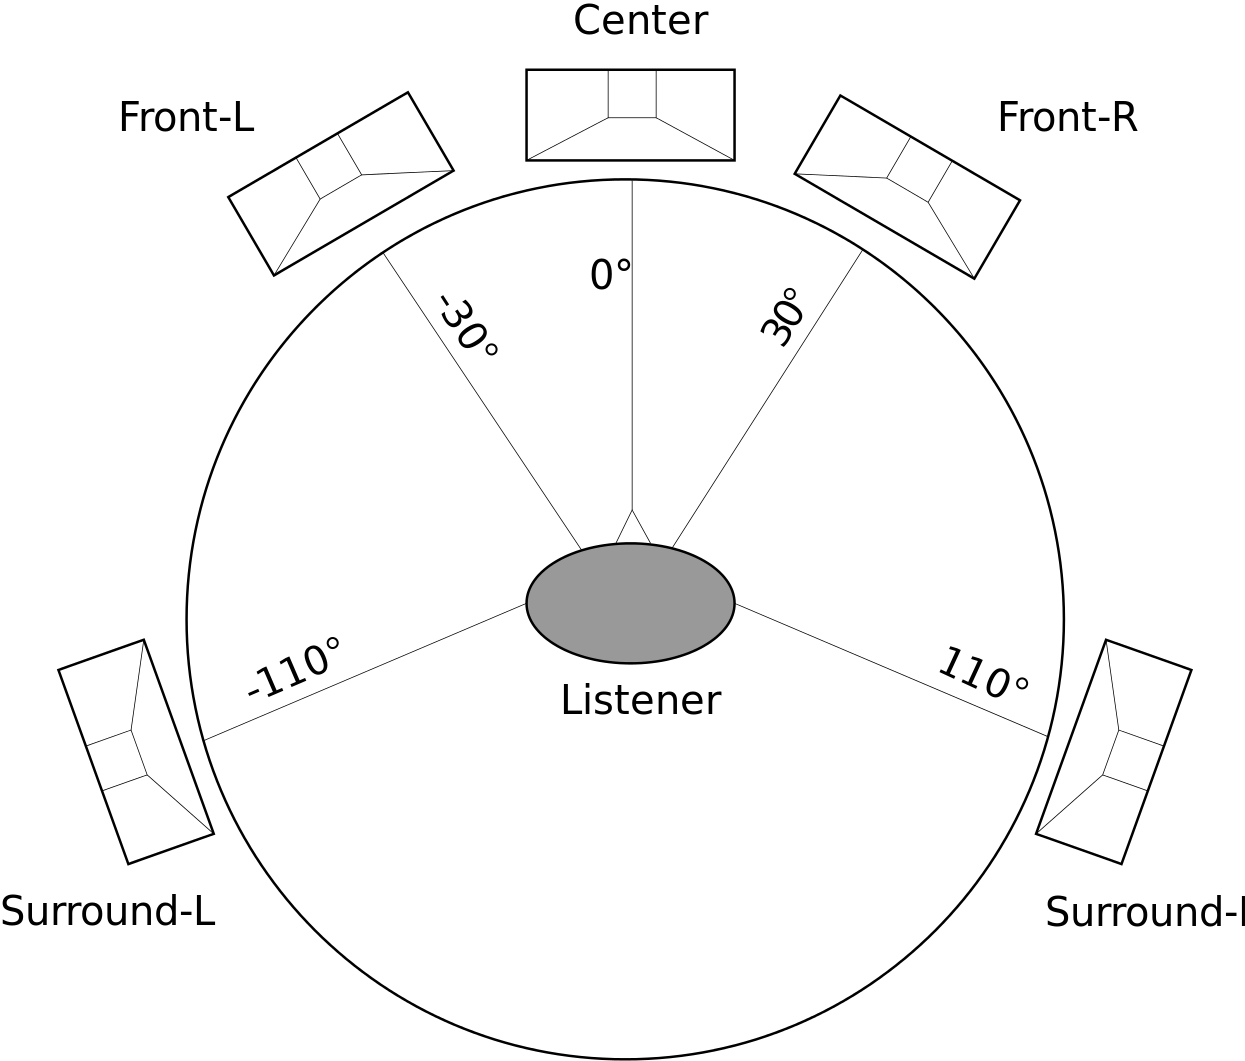
\includegraphics[scale=0.18]{figures/5-1.png}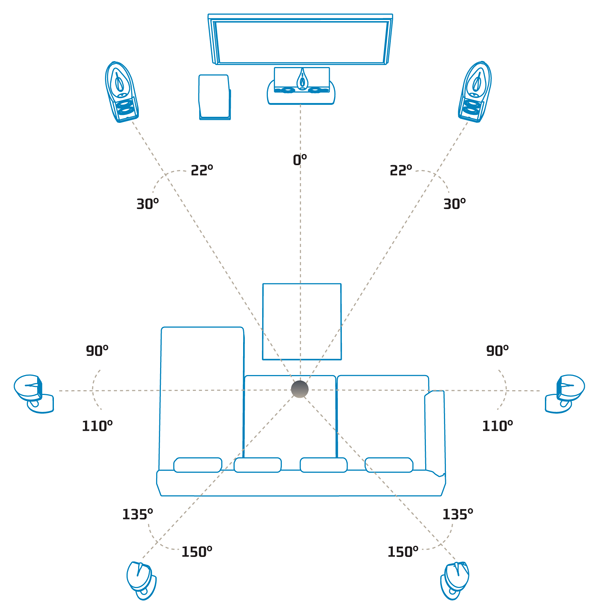
\includegraphics[scale=0.34]{figures/7-1.png}
	\caption {Configurazione 5.1 e 7.1} 
	\label{fig:5.1}
	\end{figure}
  
In parallelo una configurazione che trova il suo utilizzo nel campo della ricerca musicale e in minor misura nell'ascolto di musica è la \textbf{quadrifonia}; questa tecnica prevede l'utilizzo di 4 speaker posti sui vertici di un quadrato (angoli di $\pm45°$ e $\pm135°$) con al centro l'ascoltatore, anche questa permette una ricostruzione totale sul piano orizzontale ma ha il vantaggio di avere gli angoli tra gli speaker uguali ($90°$) il che rende più semplice un'ipotetica elaborazione di segnale per pilotarla\\

Un successivo utilizzo di questa tecnica è stata sviluppata implementando otto altoparlanti ad angoli rispettivi di $45°$ il che pone questi ultimi a $\pm22,5°\ , \pm67,5°\ , \pm112,5°\ , \pm157,5°$ come in figura \ref{fig:quadrifonia}
 
\begin{figure}[htbp]
	\centering
	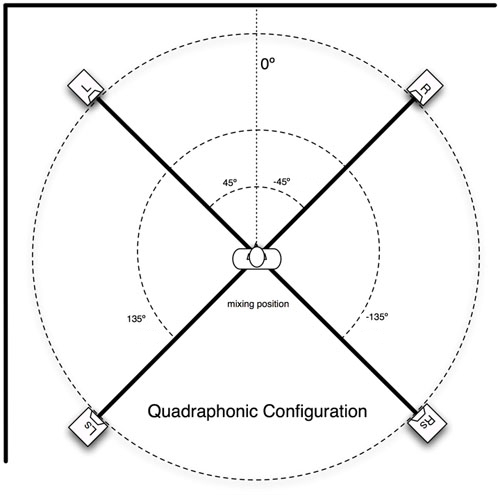
\includegraphics[scale=0.35]{figures/quad.jpg}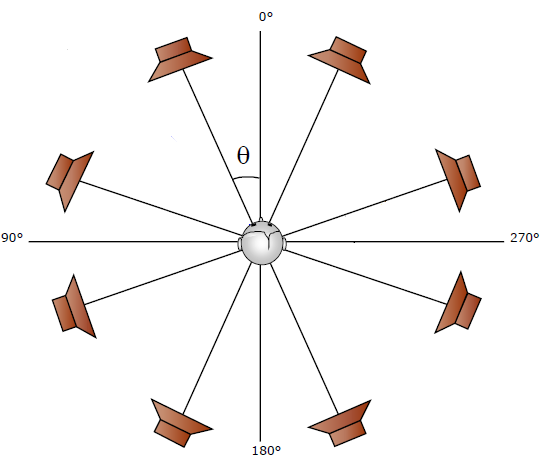
\includegraphics[scale=0.55]{figures/ottofonia.png}
	\caption {Configurazione quadrifonica e ottofonica} 
	\label{fig:quadrifonia}
	\end{figure}

\subsection{Audio in tre dimensioni}

Per finire possiamo introdurre anche l'altezza nelle nostre configurazioni, infatti sempre più spesso anche nell'uso commerciale (soprattutto nei cinema e ora anche negli home cinema) si cominciano ad utilizzare anche speaker posti sopra l'ascoltatore in modo da riprodurre oggetti sonori provenienti da quella direzione, un'esempio commerciale che da bene l'idea è la tecnologia Dolby Atmos (si veda nel paragrafo \ref{dolby} la spiegazione di quest'ultimo) ma noi, per scopi accademici, prendiamo come esempio la disposizione ottofonica tridimansionale composta da 2 piani orizzontali quadrifonici con speaker posti al di sopra e al di sotto dell'ascoltatore ad angoli di $\pm45°$ e $\pm135°$ e con elevazione di $\pm 45°$ come in figura \ref{fig:ottofonia}

\begin{figure}[htbp]
	\centering
	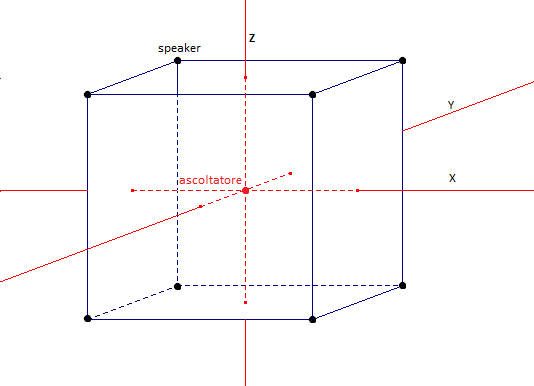
\includegraphics[scale=0.70]{figures/cubo4.png}
	\caption {Configurazione ottofonica tridimensionale} 
	\label{fig:ottofonia}
	\end{figure}

\section{Stream audio object-oriented}

Ora capito quali sono i principali standard di riproduzione andremo a spiegare come come queste configurazioni andranno pilotate, non ci interessa tanto il contenuto di ogni canale ma il fatto che: 

\begin{itemize}
\item nel più semplice dei casi ad ogni speaker sarà assegnato un canale audio differente (esempio Dolby Digital 5.1 dove ad ogni altoparlante è pilotato da un segnale discreto indipendente), si veda \cite{digital}.
\item nei casi più complessi ad ogni altoparlante sarà assegnato un mix di canali dato da una matrice di decodifica proprietaria (esempio si guardi il funzionamento del decoder Dolby Pro Logic), si veda \cite{prologic}.
\end{itemize}

Un'altra importante considerazione è il fatto che lo stesso format che utilizzo in un sistema "di grado maggiore" per esempio un 5.1 posso "scalarlo in un sistema "di grado minore" esempio uno stereo, questo perchè essendo tutti questi degli standard è possibile fare un downgrade dello stream oppure un upgrade (solo però sotto alcuni artifici) per essere adattato al sistema di riproduzione; allora viene da chiedersi perchè cambiare concenzione e approdare in uno stream object-oriented?\\

La domanda trova facile risposta nel fatto che questi giochi di upgrade o downgrade si possono fare solo su sistemi che hanno una certo grado di compatibilità (ad esempio i sistemi Dolby) e se questo avvenisse dovrei comunque prendere un format, codificarlo in un format diciamo "generale" e riadattarlo decodificandolo nel format che piloterà la mia riproduzione.\\

Allora la domanda sorge spontanea, perchè non creare uno format audio generale?\\

La Dolby laboratories ha già implementato una tecnologia che risponde in questa domanda, infatti nel suo ultimo brevetto \textbf{Dolby Atmos} (si veda documentazione \cite{atmos}) ha implementato nello stream di riproduzione anche una parte dedicata agli oggetti sonori, infatti oltre ad avere un tappeto sonoro dato dalla configurazione 7.1, la configurazione dolby atmos permette la creazione di 128 oggetti indipendenti nello spazio sonoro 3D che vengono riprodotti grazie anche all'ausilio di speaker posti al di sopra dell'ascoltatore, ma non ci soffermeremo troppo su questa configurazione, piuttosto spenderemo tempo a parlare di come Dolby é riuscita incanalare gli oggetti e la relativa informazione spaziale dentro questo stream.\\

Normalmente quando si crea un prodotto in fase di post-produzione si fa un down-mix del prodotto per passare dal contenuto dei singoli canali allo stream di riproduzione, per esempio chiudendo un mix in uno studio di registrazione classico miscelo i vari canali nello stream audio stereo con peso costituito dalla funzione di panpot deciso per ogni canale, questo succede anche in configurazioni più complicate come il 5.1 l'unica differenza è che panpot non sarà più in una dimensione ma in due\footnote{esiste una funzione di panpot standard per ogni configurazione di riproduzione}.\\

L'idea della Dolby invece è stata quella di fermarsi prima della fase di downmix (almeno per quanto riguarda il contenuto degli oggetti sonori) e di intraprendere una strada diversa:\\

Prima di tutto si devono preparare gli oggetti sonori esattamente come si vuole siano riprodotti, in secondo luogo si dispongono questi oggetti in uno spazio di riproduzione virtuale creato appositamente da un qualche software o plugin nel quale a ogni oggetto verrà assegnato un punto preciso nello spazio attraverso delle coordinate spaziali.

Questo sostanzialmente sta alla base dell'audio ad oggetti, nel prossimo capitolo vedremo come concretamente implementare questo nuovo procedimento.



\chapter{Spazilizzatore 3D e Format MDA}\label{dolby}

In questo capitolo andremo a spiegare concretamente come possiamo creare questo stream audio ad oggetti e come in fase di post produzione posso spazializzare il mio contenuto sonoro.\\

Come accennato prima in fase di post-produzione non usiamo più il solito panner installato in banchi mixer o in sofware DAW in quanto essi sia che siano stereo o 5.1 o quello che vogliamo, non hanno una spazializzazione a oggetti quindi la cosa da fare è implementare un software apposito che, sotto forma di stand-alone o di plug-in, dia in uscita gli oggetti sonori con la loro relativa posizione (in realtà oltre che alla posizione bisognerà tener conto anche di altri paramentri come grandezza, volume ecc...).\\

Parlando fino ad ora di Dolby è plausibile che prenderemo come panner 3D e come format\footnote{per format intendo lo stesso concetto che in procedenza ho usato con la parola stream} quello proprietario di Dolby Atmos ma il fatto è che essendo questa tecnica di spazializzazione soggetta a brevetto, essa é diciamo chiusa a sole applicazioni che riguardano il mondo Dolby, altri marchi hanno prodotto format proprietari simili ma sempre vincolati al brevetto, format quali Auro3D per citarne uno.\\

Noi invece ricerchiamo qualcosa che sia un format open e libero in grado di adattarsi e a diventare uno standard; la \textbf{Digital Theater System DTS} (storica rivale di Dolby) anche lei interessata all'audio ad oggetti ha creato un format open che fa al caso nostro: questo si chiama \textbf{Multi-Dimesional Audio MDA}.\\

\section{Format MDA}

Si veda \cite{mda} per la documentazione riguardante questo paragrafo.\\

Il gioco che sta alla base di questo format è la scrittura di \textbf{metadati} contenenti gli attributi dell'oggetto sonoro da spazializzare, questo format essendo principalmente stato creato per il cinema avrà attributi che per la sola riproduzione musicale sono non necessari ma di questo ne parleremo dopo.\\

Questi attributi sono:
\begin{itemize}\label{aaa}
\item \textbf{Coordinate Sferiche}: sono un set di 3 valori che indicano la posizione dell'oggetto sonoro in relazione con la posizione dell'ascoltatore che avrà come valori la terna (0,0,0).\\

Come sistema di coordinate abbiamo l'asse $X$ posto di fronte all'ascoltatore, l'asse $Y$ posto di fianco e l'asse $Z$ posto verso l'alto, quindi definiti i valori $x,y$ e $z$ su queste rette possiamo ricavare un angolo di azimut $\theta$, un'angolo di elavazione $\phi$ e un raggio $r$
posso trasformare le coordinate cartesiane in sferiche in questo modo:

\begin{equation}
	\left\{\begin{matrix}
x= r\ cos(\theta) cos(\phi) \\
y= r\ sin(\theta) cos(\phi)\\
z= r\ sin(\phi)\\
\end{matrix}\right. \ \ \Rightarrow \ \  \left\{\begin{matrix}
\theta = arctg \left(\dfrac{y}{x} \right) \\
\phi   = arctg \left(\dfrac{\sqrt{x^2 + y^2 }}{z} \right) \\
r = \sqrt{x^2 +y^2 +z^2 }\\
\end{matrix}\right.
	\label{eq:coordinatepolari}
\end{equation}

\begin{figure}[htbp]
	\centering
	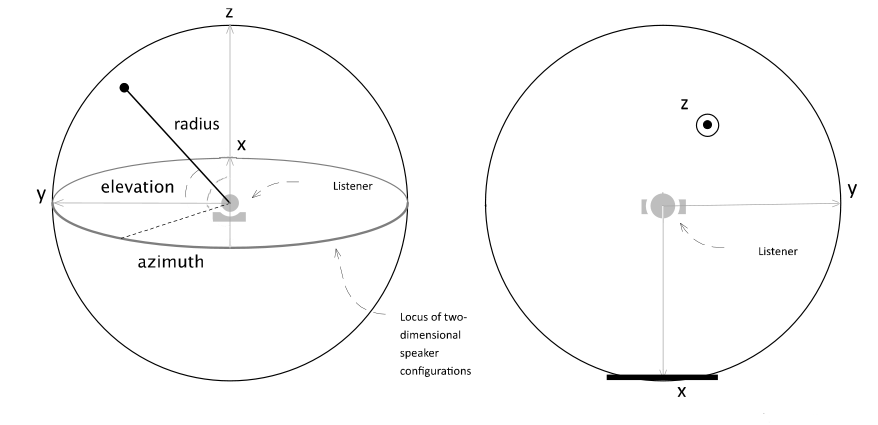
\includegraphics[scale=0.35]{figures/azimut.png}
	\caption {Coordinate spaziali} 
	\label{fig:coordinate}
	\end{figure}
	
\item \textbf{Identificativo oggetto sonoro}: scritto come URI é un numero (int) che identifica l'oggetto sonoro, sarebbe come un indirizzo.
\item \textbf{Gain}: è un valore che indica la quantità di segnale che deve avere l'oggetto sonoro.
\item \textbf{apertura}: scritta in gradi indicherebbe la grandezza dell'oggetto sonoro da ricreare(più l'oggetto è grande più gli altoparlanti posti marginalmente della sorgente fantasma si attivano, esempio se il valore è 180° allora si attiverebbero tutti i diffusori)
\item \textbf{divergenza}: anch'essa indicata in gradi quantifica la grandezza che deve avere l'oggetto sonoro ma solo sul piano orizzontale, un esempio più esplicativo si ha in figura \ref{fig:apertura}.
	
	\begin{figure}[htbp]
	\centering
	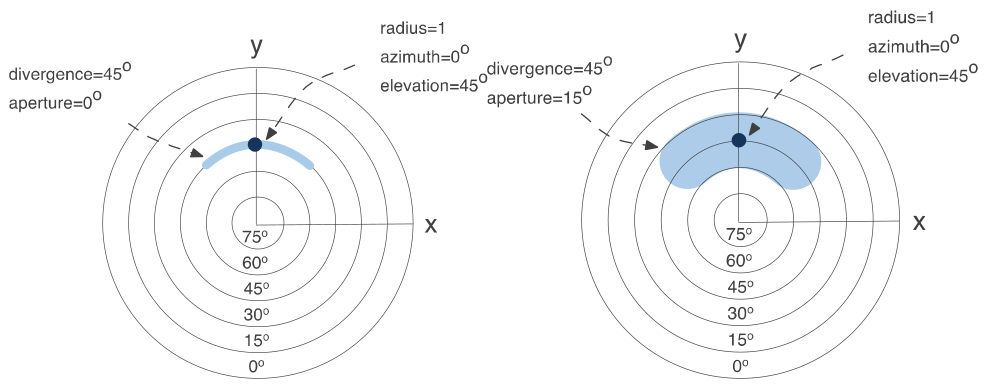
\includegraphics[scale=0.35]{figures/apertura.png}
	\caption {parametri di apertura e divergenza} 
	\label{fig:apertura}
	\end{figure}
	
	
\end{itemize}

questi sono i principali parametri scritti nei metadati che ci servono per la spazializzazione, abbiamo quindi un  oggetto sonoro e i suoi metadati ma è facile pensare che se l'oggetto si muove nello spazio o cambia dimensioni il contenuto dei suoi matadati cambia nel tempo, quindi il format racchiude in un nuovo oggetto chiamato "\textbf{Object-Fragment}" tutti i metadati descritti sopra (che per tutto lo svolgimento temporale dell'object fragment rimarranno inalterati) con più l'aggiunta di alcuni parametri come l'\textbf{ID} (identificativo oggeto), e i sample dell'oggetto sonoro da riprodurre.\\

Sopra tutto poi c'è una timeline (figura \ref{fig:time}) che ha la funzione di richiamare gli object-fragment quando servono, essa è suddivisa in segmenti temporali che sono dati da $\dfrac{1}{f_c}$ dove $f_c$ è la frequenza di campionamento impostata per la totalità degli oggetti sonori, e dove a ogni segmento è associato una lista di ID che richiama oggetti da riprodurre, un'esempio esplicativo è dato dallo schema \ref{fig:object}.\\

\begin{figure}[htbp]
	\centering
	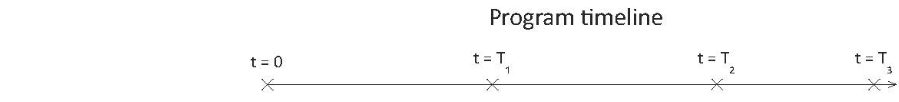
\includegraphics[scale=0.50]{figures/timeline.png}\\
	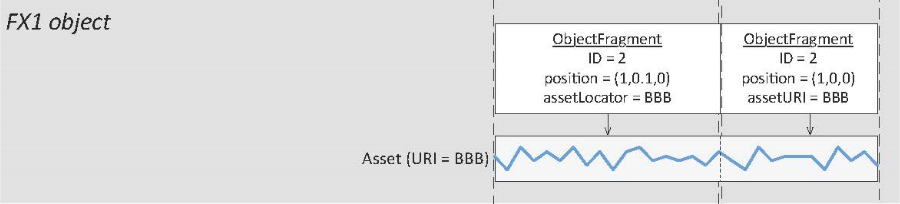
\includegraphics[scale=0.50]{figures/object1.png}\\
	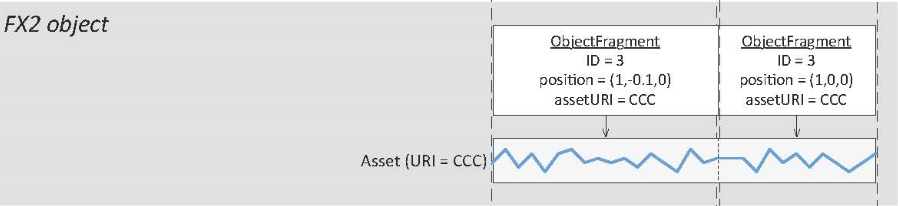
\includegraphics[scale=0.50]{figures/object2.png}\\
	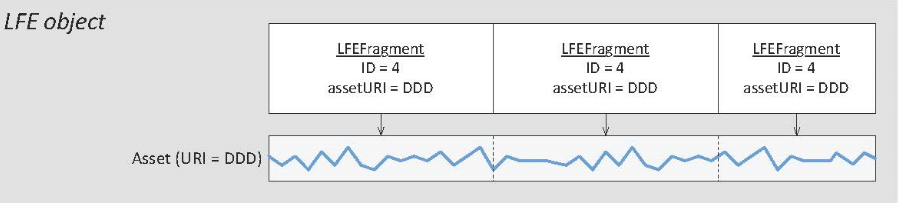
\includegraphics[scale=0.50]{figures/object3.png}
	\caption {Schema esplicativo funzionamento format MDA} 
	\label{fig:object}
	\end{figure}

\begin{figure}[htbp]
	\centering
	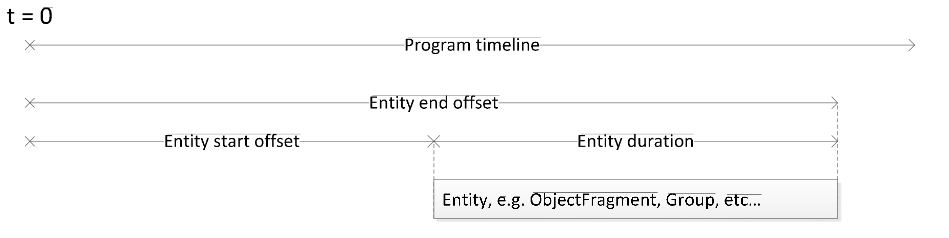
\includegraphics[scale=0.50]{figures/timeline2.png}
	
	\caption {azione di richiamo di un object-fragment} 
	\label{fig:time}
	\end{figure}

Da notare che è presente anche un LFE-Object in cui non è segnata la posizione, questo perchè data la natura omnidirezionale delle basse frequenze non avrebbe senso collocarle spazialmente e anche perchè solo il/i subwoofer sono in grado di riprodurre tali frequenze.

\subsection{Format MDA per riproduzione audio}

Qui faccio una piccola annotazione personale, nella maggior parte dei casi quando si fa musica in studio di registrazione è abbastanza difficile che abbiamo oggetti sonori in movimento e di dimensioni che variano nel tempo, quindi si potrebbe fare una piccola modifica al format in modo da alleggerire il succesivo rendering per creare fisicamente lo spazio sonoro.\\

Sostanzialmente abbiamo tre tipi di oggetti sonori in musica: oggetti fermi, oggetti che "balzano" tra due punti spaziali ed oggetti costituiti da effetti vari (il più importante per la spazializzazione è il riverbero e per questo ci occuperemo solo di questo).

tutti questi oggetti possono essere pensati come oggetti statici quindi che hanno coordinate spaziali e dimensioni fisse, in questo caso si potrebbe alleggerire il format in quanto non avrebbe più senso parlare di object-fragment (ricordiamo che gli attributi di spazializzazione cambiano allora si avranno diversi object-fragment, uno per ogni configurazione spaziale) in quanto per l'intera esecuzione del brano si avrebbe solo un object-fragment che fissa la posizione e la grandezza dell'oggetto, quindi si possono direttamente assegnare queste due ultime all'oggetto sonoro senza passare per ulteriori sottodivisioni.\\

per quanto riguarda gli oggetti statici questo trucco calza alla perfezione, per il riverbero per esempio basterà avere come oggetto il solo contenuto del brano riverberato e assegnarli una giusta divergenza e apertura; per quanto riguarda gli oggetti "balzanti" (come potrebbe essere per esempio un tremolo fatto con un pan-pot in una tastiera) basterà creare in fase di post-produzione due oggetti diversi che hanno lo stesso contenuto sonoro e che differiscono soltanto per il fatto che l'intensità sonora $I'=\alpha I$ di un'oggetto corrisponderà a una intensità $I''=(1-\alpha) I$ del secondo oggetto (dove $I$ é l'intensità totale che dovrebbe avere originariamente l'oggetto).

\section{Spazializzatore 3D}

Precedentemente abbiamo visto come è costituito il format MDA ora non ci rimane di piegare produrre materiale compatibile con questo format.\\

Nel workflow di produzione di materiale audio 3D bisognerà fermarsi quindi prima del mixdown (sia che sia stereo, 5.1 ecc...) e bisognerà prendere un qualche software che sia in grado di sostituire il mio mixer e sostituirlo con uno 3D, diverse aziende stanno sviluppando software di questo tipo in quanto vogliono interfacciarsi a questo format ed in qualche modo creare un collegamente tra il loro format proprietario e l'MDA; per esempio la Dolby ha un panner 3D per Dolby Atmos che si interfaccia con l'MDA, anche la Auro Technologies ha adottato la stessa politica o in alternativa la casa Fairlight ha creato uno spazializzatore di nome 3DAW (secondo me molto interessante) che supporta anche essa l'MDA.\\

Detto questo ho ricercato uno spazializzatore adatto e la mi ascelta è ricaduta proprio sull'\textbf{MDA creator} proprietaria della DTS in quanto è la più intuitiva e la miglior scelta per integrazione (in quanto essa ha creato sia il panner che il format).

\begin{figure}[htbp]
	\centering
	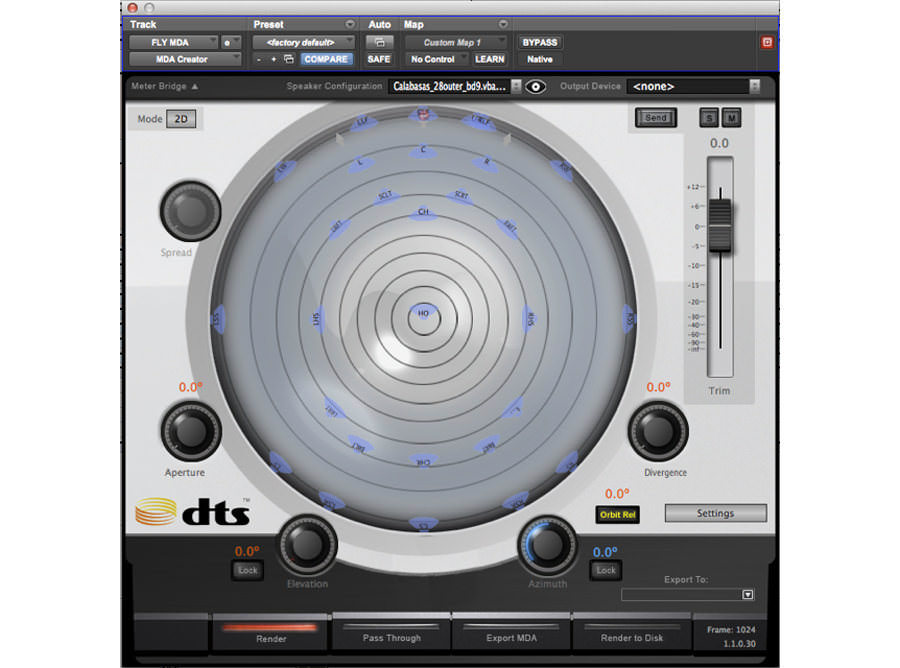
\includegraphics[scale=0.50]{figures/mdacreator.jpg}
	
	\caption {MDA Creator, DTS technology} 
	\label{fig:mdacreator}
	\end{figure}

Tutte le informazioni su MDA creator verranno prese dal suo manuale \cite{creator}.\\

questo plugin disponibile solo per Protools è di semplice comprensione, come da manuale bisogna mettere in insert in ogni traccia questo plugin (condizione necessaria è che tutte le tracce devono avere la stessa lunghezza), poi aprendo l'interfaccia del panner bisognerà posizionare ogni oggetto nel punto in cui si desidera e con divergenza e apertura voluta (si veda il paragrafo \ref{aaa} per sapere i parametri del format), logicamente questi parametri possono essere automatizzati per spostare e modificare l'oggetto nel tempo.

Inoltre si possono creare dei "Bed Object" che sarebbero oggetti i quali vengono direttamente codificati nel sistema di riproduzione scelto (esempio classico è la colonna sonora in 5.1 nei film) ai quali verranno sommati gli oggetti veri e propri del format e l'LFE-Object per gli effetti a bassa frequenza.\\

Una volta fatto questo l'MDA creator metterà a disposizione tre scelte di output, quella che interessa a noi è la modalità di esportazione con mda file: questa scelta ci porta alla creazione dei file \textbf{.map, .mix} e \textbf{.mda}, quest'ultimo è proprio il file contenente i metadati e gli oggetti sonori proposti in questo format.


\chapter{Decodifica format MDA per adattamento a varie configurazioni}

In questo capitolo parleremo invece di come da un format MDA posso passare a una configurazione di riproduzione usuale, mediante la tecnica VBAP.\\

\section{Tecnica VBAP}
 
Il \textbf{Vector Base Amplitude Panning VBAP} è una tecnica di spazializzazione che permette di localizzare una sorgente sonora attraverso la differenza di intensità emessa tra due o più speaker, mi spiego meglio:\\
uno dei due parametri con cui il nostro cervello discrimina la direzione di una sorgente è la IID (si veda \cite{iid}) che indica la differenza di intensità che le nostre orecchie devono percepire per far si che si percepiamo una sorgente fantasma in un punto dello spazio, quindi se riproduciamo un segnale coerente (cioè in fase fra gli altoparlanti) con minimo di due speaker e gli riproduciamo con intensità diverse, allora ci sembrerà di sentire il segnale proveniente da un punto previsto dalla IID.\\

Ora la cosa diventa abbastanza semplice in quanto se volgiamo ricreare una spazializzazione 2D basteranno due speaker, se invece vogliamo fare un 3D allora serviranno un minimo di 3 speaker posti a triangolo, configurazioni del genere esistono già e sono state ampiamente testate ed affinate, per tutta la documentazione riguardante il VBAP si faccia riferimento a \cite{vbap}.\\

E' d'obbligo affrontare un po di matematica per riuscire poi ad adattare il VBAP alle configurazioni esposte in \ref{metodi}, partiamo subito con il caso bidimensionale con 2 speaker affrontando la cosa direttamente con calcolo matriciale (all'inizio più difficile ma meglio generalizzabile per dopo).\\

\subsection{VBAP 2D}\label{c}
Consideriamo un sistema fatto da due monitor, definiamo ora arco attivo la porzione di arco compresa tra i due speaker, ora conoscendo la posizione della nostra sorgente virtuale collocata in punto dell'arco attivo (cosa che si adatta esattamente al nostro caso) l'unica cosa che non sappiamo sono i gain $g_1$ e $g_2$ da applicare ad ogni segnale che vanno rispettivamente alle due casse per ricostruire esattamente lo spazio sonoro, quindi definendo un sistema di riferimento cartesiano $ \boldsymbol{X},\boldsymbol{Y}$ definirò come $ \boldsymbol{l_{1}}= {\left[ l_{11} \ l_{12} \right]}^T \ \  \boldsymbol{l_{2}}= {\left[ l_{21} \ l_{22} \right]}^T$ i vettori unitari che puntano verso i due altoparlanti e $\boldsymbol{p}= {\left[ p_1 \ p_2 \right]}^T$ il vettore unitario che punta verso la sorgente virtuale.\\ 

\begin{figure}[htbp]
	\centering
	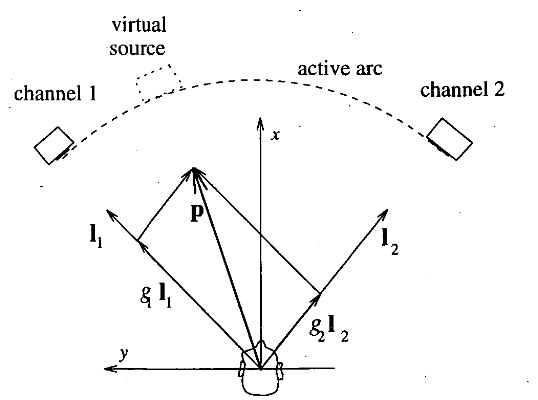
\includegraphics[scale=0.40]{figures/matrix2d.png}
	\caption {composizione vettoriale delle sorgenti reali e virtuale} 
	\label{fig:vettori2d}
	\end{figure}

Il trucco ora sta nel fatto che posso riscrivere il vettore $\boldsymbol{p}$ in funzione del vettore contenente i due gain $\boldsymbol{g}= \left[ g_1 \ g_2 \right]$ come:

\begin{equation}
\boldsymbol{p}= \boldsymbol{g} \cdot \boldsymbol{l} = \left[g_1 \ g_2 \right] \left[\boldsymbol{l_{1}} \ \boldsymbol{l_{2}} \right]^T = g_1 \boldsymbol{l_{1}} + g_2 \boldsymbol{l_{2}}
\label{eq:bbbb}
\end{equation}

In questo caso però possiamo ulteriormente compattare la scrittura in quanto:

\begin{equation}
\boldsymbol{p}=g_1 {\left[ l_{11} \ l_{12} \right]}^T + g_2 {\left[ l_{21} \ l_{22} \right]}^T= \left[ g_1 \ g_2 \right] \left[\begin{matrix}
l_{11} & l_{12}\\ l_{21} & l_{22}
\end{matrix} \right]
\label{eq:cccc}
\end{equation}

ora trovando tutto in funzione $g$ abbiamo che:

\begin{equation}
\left[g_1 \ g_2\right] = \left[ p_1 \ p_2 \right]  {\left[\begin{matrix} 
l_{11} & l_{12}\\ l_{21} & l_{22}
\end{matrix} \right]}^{-1} \ \ \Rightarrow \ \ \ \boldsymbol{g}=\boldsymbol{p}^T {\boldsymbol{L_{12}}}^{-1}
\label{eq:dddd}
\end{equation}

Logicamente assumo che la matrice $\boldsymbol{L_{12}}$ ammetta l'inversa, ora parametrizzo tutto in funzione di $\theta$ e $\theta_0$ nel modo seguente: 

\[ p_1=cos(\theta),\ p_2=sen(\theta),\ l_{11}=cos(\theta_0),\ l_{12}=sen(\theta_0),\ l_{21}=cos(-\theta_0),\ l_{22}=sen(-\theta_0) \]

\begin{figure}[htbp]
	\centering
	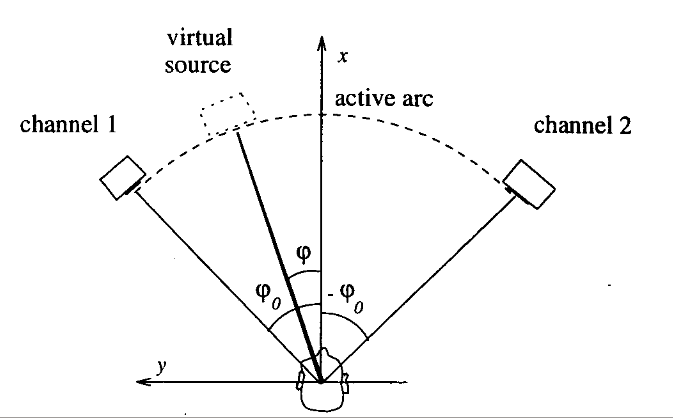
\includegraphics[scale=0.40]{figures/angoli.png}
	\caption {angoli delle sorgenti reali e virtuale} 
	\label{fig:angoli}
	\end{figure}

fatto questo, essendo il nostro spazio ortogonale, posso calcolare direttamente i coefficienti dei due gain invertendo prima la matrice, il risultato è il seguente:

\begin{equation}\begin{split}
g_1=\dfrac{cos(\theta) sen(\theta_0) + sen (\theta) cos(\theta_0)}{2 cos(\theta_0) sen(\theta_0)}\\ \\
g_2=\dfrac{cos(\theta) sen(\theta_0) - sen (\theta) cos(\theta_0)}{2 cos(\theta_0) sen(\theta_0)}
\end{split}
\label{eq:eeee}
\end{equation}

Logicamente introduciamo un coefficente $C$ che indica il gain complessivo (ci servirà per definire la distanza dell'oggetto) e che scalerà i nosti due gain in questo modo:

\begin{equation}
\left[g_1 \ g_2\right]_{scaled} = \dfrac{\sqrt{C} \left[ g_1 \ g_2 \right]}{\sqrt{g_1^2 + g_2^2}} 
\label{eq:ffff}
\end{equation}

Sarebbe molto limitativo usare questa tecnica per ricreare una riproduzione stereo, infatti con qualche accorgimento nulla ci vieta di poter estendere ad $n$ diffusori questa tecnica, l'unica accortezza è che il nostro procedimento dovrà "selezionare" solo due speaker alla quale attribuire la realizzazione della sorgente virtuale, questa scelta si basa sulla posizione dell'oggetto infatti quest'ultimo potrà essere messo solo in un'arco attivo (l'intero arco giro è suddiviso in archi attivi che non si sovrappongono) quindi le due casse che delimitano questo arco, saranno la coppia imputata a svolgere la riproduzione; faccio un piccolo esempio:\\

consideriamo come numero $n$ arbitrario di casse consecutive $a_n$ disposte ad un angolo $\theta_{0,n}$ tali che $0°\leq \theta_{0,1},\ \theta_{0,2},\ \ldots,\ \theta_{0,n} <360°$, posizionando un qualsiasi oggetto virtuale in un qualsiasi angolo $\theta^{\prime}$ dovrà verificarsi che $\theta_{0,m}\leq \theta^{\prime} \leq \theta_{0,m+1}$ dove $m$ sta per il numero dello speaker adiacente alla sorgente virtuale ma con angolazione minore, quindi in questo caso la coppia di casse da selezionare saranno $a_m$ e $a_{m+1}$, quindi per rendere effettivo il metodo descritto nel caso di due speaker dovremo fare una piccola modifica in quanto dovremo assumere: 

\begin{equation}
\theta_0 = \dfrac{\theta_{0,m+1}-\theta_{0,m}}{2} \ \ \ \ \ \theta=\theta^{\prime}-\dfrac{\theta_{0,m+1}+\theta_{0,m}}{2}
\label{phidiverso}
\end{equation}

   
 \begin{figure}[htbp]
	\centering
	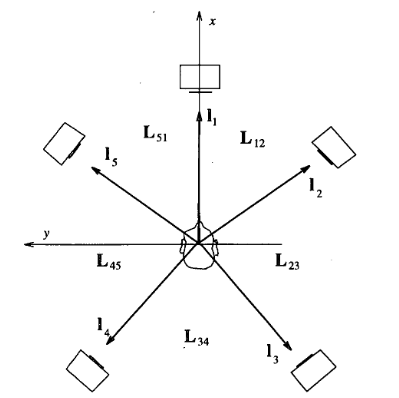
\includegraphics[scale=0.50]{figures/matrix5-1.png}
	\caption {VBAP nidimensionale con più altoparlanti} 
	\label{fig:angoli5}
	\end{figure}
  
   
   
\subsection{VBAP 3D}

Capito qual'è il modello e l'algoritmo di implementazione del VBAP in due dimensioni estenderemo il concetto in tre dimensioni.\\

La più piccola configurazione di tre altoparlanti consiste nel disporli ai vertici di un triangolo equilatero come in figura \ref{fig:triangolo}, quindi ora basta prendere la formule usate sopra ed estenderle con la dimensione $\boldsymbol{Z}$ introducendo quindi l'angolo $\phi$ che indica l'elevazione dal piano orizzontale.

\begin{figure}[htbp]
	\centering
	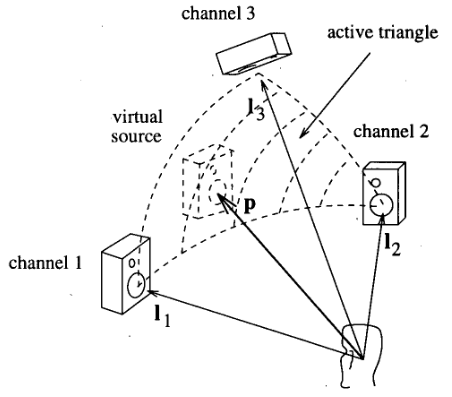
\includegraphics[scale=0.40]{figures/matrix3d.png}
	\caption {composizione vettoriale delle sorgenti reali e virtuale in tre dimensioni} 
	\label{fig:triangolo}
	\end{figure}

E' logico anche che la sorgente virtuale potrà essere collocata soltanto nella calotta\footnote{con calotta si intende una porzione di superficie di una sfera} delimitata dalle rette congiungenti gli altoparlanti a due a due,	 quindi esattamente come sopra se definiamo i vettori unitari che puntano alle tre casse come $ \boldsymbol{l_{1}}= {\left[ l_{11} \ l_{12} \ l_{13} \right]}^T \ \ \boldsymbol{l_{2}}= {\left[ l_{21} \ l_{22} \ l_{23} \right]}^T \ \ \boldsymbol{l_{3}}= {\left[ l_{31} \ l_{32} \ l_{33} \right]}^T$ e il vettore della sorgente virtuale $\boldsymbol{p}= {\left[ p_{1} \ p_{2} \ p_{3} \right]}^T$ risulta che:

\begin{equation}
\boldsymbol{p} = \boldsymbol{g} \cdot \boldsymbol{l} = \left[ g_1 \ g_2 \ g_3 \right] \left[ \boldsymbol{l_{1}} \ \boldsymbol{l_{2}} \ \boldsymbol{l_{3}} \right]^T
\label{gggg}
\end{equation}

quindi ribaltando l'equazione ci rimane che:

\begin{equation}
\left[g_1 \ g_2 \ g_3 \right] = \left[ p_1 \ p_2 \ p_3 \right]  {\left[\begin{matrix} 
l_{11} & l_{12} & l_{13}\\ l_{21} & l_{22} & l_{23} \\ l_{31} & l_{32} & l_{33}
\end{matrix} \right]}^{-1} \ \ \Rightarrow \ \ \ \boldsymbol{g}=\boldsymbol{p}^T {\boldsymbol{L_{123}}}^{-1}
\label{hhhh}
\end{equation}

anche in questo caso possiamo calcolare i tre coefficienti scalati in questa maniera:

\begin{equation}
\left[g_1 \ g_2 \ g_3 \right]_{scaled} = \dfrac{\sqrt{C} \left[ g_1 \ g_2 \ g_3 \right]}{\sqrt{g_1^2 + g_2^2 + g_3^2}} 
\label{iiii}
\end{equation}

in questo caso fare un'esempio non è possibile in quanto il VBAP in tre dimensioni è molto legato alla geometria di implementazione e la trigonometria sulla sfera è analiticamente pesante anche se possibile, quindi si preferisce lasciare al calcolatore il compito del calcolo vettoriale senza lasciare a noi il compito di tradurre il tutto in funzioni angolari, si veda per esempio il passaggio dalla formula \ref{eq:dddd} alla formula \ref{eq:eeee}.\\

Ora, come sopra, possiamo arrivare ad un numero $n$ di altoparlanti per coprire tutto l'angolo solido, anche qui il nostro algoritmo dovrà "selezionare" gli altoparlanti che saranno imputati alla riproduzione del nostro oggetto sonoro, gli stessi che delimiteranno la calotta attiva che racchiude la sorgente virtuale.

\begin{figure}[htbp]
	\centering
	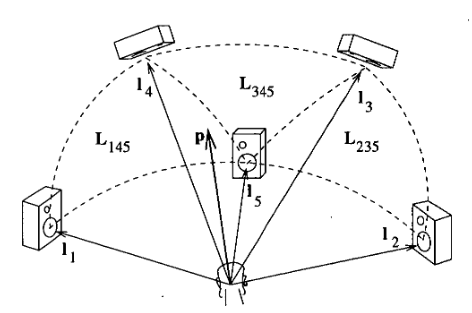
\includegraphics[scale=0.40]{figures/matrix3dfull.png}
	\caption {configurazione a più altoparlanti per la tecnica VBAP in tre dimensioni} 
	\label{fig:matrix3dfull}
	\end{figure}


\section{Integrazione del formato MDA con la tecnica VBAP}

Ricapitolando siamo arrivati al punto di sapere cos'è il format MDA e che cos'è la tecnica di spazializzazione VBAP, 
il passo successivo è riuscire ad integrare i due insieme, la cosa non è difficile ma procediamo per gradi.\\

N.B) nel corso di questo capitolo
ricordiamo che il format MDA contiene oggetti sonori a cui vengono associati metadati contenenti posizione nelle tre dimensioni e grandezza, essi devono essere spacchettati e adattati in modo da essere letti dall'algoritmo del VBAP.\\

Un concetto fondamentale da capire è che essendo le informazioni, nei metadati, relative a uno spazio tridimensionale, esse si adatteranno benissimo a una riproduzione VBAP tridimensionale con la somma delle calotte attive coprenti l'intera superficie sferica in cui è immerso l'ascoltatore, se il tipo di riproduzione non è questo allora bisognerà adattare i metadati in modo da poter essere congruenti all configurazione che andranno a pilotare, logicamente queste trasformazioni dovranno il più possibile lasciare inalterata la percezione spaziale a quella che è stato decisa in fase di post-produzione.\\

andremo ora a vedere come integrare le due cose per alcune delle le configurazioni del capitolo \ref{metodi}

\subsection{Utilizzo MDA in geometrie tridimensionali}

Per prima cosa facciamolo per le geometrie tridimensionali infatti per queste non c'è bisogno di fare delle trasformazioni sulle coordinate in quante esse possono essere applicate direttamente, l'unica cosa che c'è da fare è un piccolo discorso sulle distanze e sui raggi.\\

Introduciamo due raggi, $r_0$ che sarebbe la lunghezza del vettore congiungente l'ascoltatore con uno degli speaker (non importa quale dato che tutti gli speaker sono posizionati sulla superficie di una sfera quindi si avranno tutti raggi uguali) e definiamo $r_1$ come la lunghezza del vettore congiungente l'ascoltatore e il più vicino degli oggetti virtuali che si vuole creare, premettendo che io posso solo riprodurre sorgenti virtuali a partire dalla superficie della sfera verso l'esterno, allora qualsiasi di questi che avranno $r_n \leq r_0$ non sarò in grado di riprodurli nella maniera corretta, quindi dovrò attuare una trasformazione in modo da lasciare inalterata la distanza relativa fra le sorgenti virtuali in questo modo:

\begin{equation}
\left\{\begin{matrix}
se\ \  r_1 \leq r_0\ \ \Rightarrow \ \ r_n^{\prime} = r_n+(r_0 - r_1) \ \ \forall n \geq 1\\
\\
se\ \  r_1 \geq r_0\ \ \Rightarrow \ \ r_n^{\prime} = r_n\ \ \forall n \geq 1\\
\end{matrix}\right.
\label{jjjj}
\end{equation}

fatto questo non ci rimane che intervenire sul fattore $C$ introdotto nel paragrafo \ref{c} in quanto esso contribuisce alla sensazione di lontananza, mi spiego meglio:

Principalmente sono quattro i fattori che intercorrono alla corretta ricostruzione in lontananza di un'oggetto, essi sono l'intensità sonora, la colorazione timbrica, il rapporto riverbero/segnale diretto e il delay temporale \footnote{la spiegazione del perchè di tutti questi parametri richiederebbe molto tempo quindi diamo per buone queste assunzioni}, l'informazione relativa agli ultimi tre parametri possono essere contenute direttamente nel segnale audio dell'oggetto sonoro, invece noi dobbiamo considerare l'intensità sonora in quanto legata alla distanza dall'oggetto all'ascoltatore e quindi al suo raggio\footnote{in realtà ogni modifica del raggio si dovrebbe ripercuote anche sugli altri tre parametri cosa che nel nostro caso non avviene essendo questi ultimi tre contenuti nell'audio dell'oggetto sonoro, siamo quindi di fronte ad un'errore ma che possiamo considerare trascurabile visto l'entità ridotta delle trasformazioni sui raggi }.\\

come detto sempre nel paragrafo \ref{c} il fattore $C$ è legato al gain complessivo dell'oggetto ma quest'ultimo posizionato sulla superficie della sfera, ora sappiamo dalla formula \ref{jjjj} che ogni oggetto è posizionato o sulla sfera o al suo esterno quindi possiamo prenderci la libertà di scalare il coefficiente $C$ in base alla distanza dell'oggetto dalla sfera in questo modo:

\begin{equation}
\boldsymbol{g_{n\ scaled}} = \dfrac{\sqrt{C_n \ f^{\prime}}\ \boldsymbol{g_n}}{\sqrt{g_1^2 +g_2^2 + g_3^2}} \ \ \ con \ \ \ \left\{\begin{matrix}
f^{\prime}= \frac{arctan\left((r_n^{\prime}-r_0)\ \dfrac{\pi}{2}\right)}{(r_n^{\prime}-r_0)\ \dfrac{\pi}{2}} & per\ r_n^{\prime}>r_0
\\
f^{\prime}=1 & per\ r_n^{\prime}=r_0
\end{matrix}\right.
\label{kkkk}
\end{equation}

In teoria l'ampiezza di un segnale sonoro dovrebbe calare con l'inverso della distanza e quindi nel nostro caso come $\frac{1}{r_n^{\prime}-r_0}$ ma facendo così avremmo dei problemi di divergenza per $r_n^{\prime}=r_0$ e valori sballati per la differenza $<1$, quindi in accordo con quanto scritto in \cite{distanza} introduco una funzione $f^{\prime}$ che approssima il più possibile la funzione originale ma che risolve totalmente i problemi nelle zone difficili (figura \ref{fig:distance})\\

\begin{figure}[htbp]
	\centering
	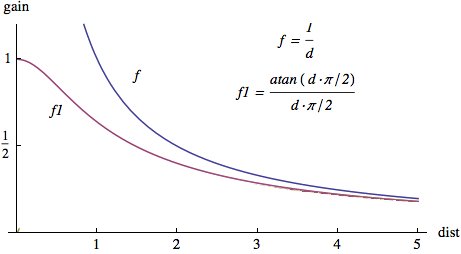
\includegraphics[scale=0.60]{figures/distance.png}
	\caption {funzione distanza originale e funzione approssimata} 
	\label{fig:distance}
	\end{figure} 

Logicamente quanto detto qui sopra dovrà essere applicato in tutti casi di VBAP sia tridimensionale che non in quanto bisogna tener conto della distanza degli speaker ed è molto difficile che si abbiano tutti gli oggetti alla stessa distanza.\\

\subsection{Utilizzo MDA in configurazioni planari}

introduciamo ora un problema aggiuntivo: come faccio a riprodurre un programma sonoro tridimensionale in un impianto planare? questa domanda è di difficile risposta in quanto la riproduzione o meno tramite il VBAP in due dimensioni dipende dalla posizione dell'oggetto, mi spiego meglio:\\

Nei metadati del format MDA sono presenti gli angoli $\theta, \phi$ e il raggio $r$ che identificano la posizione, quello che ci da informazioni sull'altezza è l'angolo (appunto detto di elevazione) $\phi$ quindi ponendo semplicemente $\phi=0°$ sulla carta elimineremmo la dimensione verticale ma comprometteremmo anche la percezione degli oggetti originariamente posti sopra l'ascoltatore.\\

Per esempio, mettiamo il caso che un oggetto sia posto ad un angolo $	\theta= 90° $ e un angolo $\phi=89°$, esso praticamente si trova quasi perfettamente al disopra della nostra testa, a primo acchito verrebbe da pensare di porre semplicemente quest'ultimo a $0$ ma si avrebbe uno spostamento netto dell'oggetto alla completa sinistra dell'ascoltatore il che è incongruente con la scelta iniziale del produttore, quindi si capisce che questa strada è concettualmente sbagliata.\\

Contrariamente un oggetto posto a $	\theta= 90° $ con un angolo $\phi=45°$ e $r=6m$ posso tranquillamente pensarlo come proveniente solamente da sinistra visto la sua distanza dall'ascoltatore, quindi riproducibile con un VBAP in due dimensioni.\\

Ma vediamo ora come faccio a selezionare gli oggetti "buoni e cattivi" per la riproduzione con il VBAP, per prima cosa sposto tutti gli oggetti della semisfera inferiore sopra l'ascoltatore in questo modo:

\begin{equation}
\phi_{n,top} = arctg  \left( \dfrac{\vert sen(\phi_n) \vert}{ cos(\phi_n) } \right)
\label{  b}
\end{equation}

Successivamente, tracciando la proiettante dell'oggetto nel piano orizzontale, si può vedere che gli oggetti che soddisfano l'equazione \ref{zzz} possono essere riprodotti con il VBAP tralasciando l'angolo azimutale e considerando le formule del capitolo \ref{c}.

\begin{equation}
r_{n,shadow}=r_n^{\prime} cos(\phi_{n,top}) \geq r_0     
\label{zzz}
\end{equation}

Tutti gli altri oggetti invece no, ma una soluzione a questi ultimi potrebbe essere di creare un ascolto immersivo per quegli oggetti sfruttando tutti gli speaker del piano di ascolto e scalando il segnale da inviare a tutti questi ultimi in base alla posizione della proiettante dell'oggetto sul piano orizzontale, nel primo caso sopra la proiettante dell'oggetto sarebbe un punto molto vicino all'ascoltatore immediatamente alla sua sinistra, quindi i due speaker a sinistra dovrebbero riprodurre la metà più un poco di potenza sonora attribuita all'oggetto, invece gli speaker a la differenza per arrivare ad uno.\\

Sicuramente una tecnica che faccia questo esiste già ma non essendo il VBAP non verrà discussa in questa tesi.






\subsection{Utilizzo MDA in geometria lineare}

Per ultimo vediamo come adattare il format alla configurazione monomensionale, ho parlato al singolare in quanto a meno di configurazioni esoteriche si utilizzerà sempre il sistema stereo posto di fronte all'ascoltatore, bisogna qui stravolgere il format in maniera pesante in quanto si devono sottrarre ben due dimensioni ma paradossalmente i passaggi da fare sono più semplici\\ 

Come prima cosa dovrò spostare tutti gli oggetti che originariamente sono posti dietro (quindi con angoli compresi tra $90°$ e $270°$) davanti all'ascoltatore operando una trasformazione sull'angolo azimutale:

\begin{equation}
\theta_{n,front} = arctg  \left( \dfrac{sen(\theta_n)}{\vert cos(\theta_n)\vert } \right)
\label{llll}
\end{equation}

In questo modo tutti gli angoli azimutali di ogni oggetto sarà posto tra $-90 \leq \theta_n \leq +90$\\

Abbiamo ottenuto oggetti posti al massimo perfettamente ai nostri fianchi ma la configurazione stereo prevede al massimo una riproduzione di oggetti a $\pm 30°$ data dalla limitata ampiezza angolare $\pm \theta_0$ degli speaker, quindi dovrò rimappare gli angoli appena ottenuti in modo da essere compresi tra $0, \pm 30°$.\\ 

Come primo approccio ho pensato semplicemente di dividere per un fattore tre gli angoli ma accade che gli oggetti posti sullo scenario frontale vengono schiacciati troppo verso l'origine degli angoli, quindi ho optato per la funzione seno (usata come peso) che schiacciasse gli oggetti posti sui lati e che lasciasse il più inalterati possibile gli angoli degli oggetti posti di fronte, in più il tutto viene ulteriormente scalato per il coseno dell'angolo di elevazione per tenere conto di quest'ultimo e della proiezione del vettore sul piano orizzontale, in questo modo:

\begin{equation}
\theta_{n, remapped}= \theta_0 \cos(\phi) \ sen (\theta_{n,front}) = \theta_0 \cos(\phi)\ sen \left( arctg  \left( \dfrac{sen(\theta_n)}{\vert cos(\theta_n)\vert } \right)\right)
\label{mmmm}
\end{equation}





\subsection{Esempio di integrazione con sistemi quadrifonico, 5.1 e stereo}

Per tutti gli esempi che farò vorrò riprodurre tre oggetti con seguenti coordinate sferiche per far vedere ogni caso:\\

\begin{tabular}{|c|c|c|c|c|}
\hline 
oggetto 1 & $\theta_1=15°$ & $\phi_1=0°$ & $r_1=1,5m$ & $C_1=1,3$ \\ 
\hline 
oggetto 2 & $\theta_2=275°$ & $\phi_2=0°$ & $r_2=2,5m$ & $C_2=1,6$ \\ 
\hline 
oggetto 3 & $\theta_3=160°$ & $\phi_3=45°$ & $r_3=3,0m$ & $C_1=0,8$ \\ 
\hline 

\end{tabular} \\ \\
 
N.B) ai fini dei calcoli conviene pensare $\theta_2=275°$ come $\theta_2=-85°$.\\

Cominciamo con la quadrifonia, una possibile configurazione potrebbe essere questa:\\

\begin{tabular}{|c|c|c|}
\hline 
speaker 1 & $\theta_{0,1}=45°$ & $r_0=2m$\\ 
\hline  
speaker 2 & $\theta_{0,2}=135°$ & $r_0=2m$\\ 
\hline 
speaker 3 & $\theta_{0,3}=-135°$ & $r_0=2m$\\ 
\hline 
speaker 4 & $\theta_{0,4}=-45°$ & $r_0=2m$\\ 
\hline 
\end{tabular} \\
\\

Come prima cosa applichiamo la formula \ref{jjjj} in modo da scalare i raggi degli oggetti e rendergli

\[r_1^{\prime}=2m \ \  r_2^{\prime}=3m \ \ r_3^{\prime}=3,5m  \]

Ora è facile trovare i gain e i gain scalati del primo e del secondo oggetto in quanto il primo è riprodotto dagli speaker 4 e 1 invece il secondo dagli speaker 3 e 4 in questo modo:

per entrambi gli oggetti, prima applico la formula \ref{phidiverso} in modo da trovare i nuovi angoli da mettere nella formula \ref{eq:eeee} poi considerando i coefficienti $C_n$ e i raggi $r_n^{\prime}$ ricavo dalla formula \ref{kkkk} i gain scalti per entrambi gli oggetti che in questo caso saranno:

\begin{equation}
\begin{matrix}
g_{(1,obj\ 1)} = 0,87 & g_{(1,obj\ 1)scaled} = 0,861\\ 
g_{(4,obj\ 1)} = 0,50 & g_{(4,obj\ 1)scaled} = 0,733\\
g_{(4,obj\ 2)} = 0,76 & g_{(4,obj\ 2)scaled} = 0,779\\
g_{(3,obj\ 2)} = 0,64 & g_{(3,obj\ 2)scaled} = 0,651\\
\end{matrix} 
\label{gscalatiesempio1}
\end{equation}
\\

Passiamo ora all'adattamento alla configurazione 5.1\\

Una possibile configurazione di impianto 5.1 potrebbe essere la seguente:\\

\begin{tabular}{|c|c|c|} 
\hline 
speaker 1 & $\theta_{0,1}=0°$ & $r_0=2m$\\ 
\hline 
speaker 2 & $\theta_{0,2}=30°$ & $r_0=2m$\\ 
\hline 
speaker 3 & $\theta_{0,3}=110°$ & $r_0=2m$\\ 
\hline 
speaker 4 & $\theta_{0,4}=-110°$ & $r_0=2m$\\ 
\hline 
speaker 5 & $\theta_{0,4}=-30°$ & $r_0=2m$\\ 
\hline
\end{tabular} \\

Non ci rimane che operare nella stessa maniera utilizzata per la quadrifonia esposta appena sopra (infatti si applicheranno esattamente le stesse formule con l'unica differenza di avere dei $\theta_{0,n}$ visibilmente diversi),ricavandomi così i gain e i gain scalati degli speaker 2 e 1 (imputati alla riproduzione del primo oggetto) e 5 e 4 (imputati alla riproduzione del secondo):\\

\begin{equation}
\begin{matrix}
g_{(2,obj\ 1)} = 0,52 & g_{(2,obj\ 1)scaled} = 0,806\\ 
g_{(1,obj\ 1)} = 0,52 & g_{(1,obj\ 1)scaled} = 0,806\\
g_{(5,obj\ 2)} = 0,43 & g_{(5,obj\ 2)scaled} = 0,465\\
g_{(4,obj\ 2)} = 0,83 & g_{(4,obj\ 2)scaled} = 0,898  \\
 
\end{matrix} 
\label{gscalatiesempio2}
\end{equation} \\



% qui andrebbero due parole sul terzo oggetto



Per ultimo esempio vediamo il risultato dell'adattamento alla configurazione stereo.\\

Una configurazione possibile potrebbe essere la seguente:\\

\begin{tabular}{|c|c|c|}
\hline 
speaker 1 & $\theta_{0,1}=30°$ & $r_0=2m$\\ 
\hline 
speaker 2 & $\theta_{0,2}=-30°$ & $r_0=2m$\\ 
\hline 
\end{tabular} \\

Applicando rispettivamente la formula \ref{llll} e la formula \ref{mmmm} ottengo i seguenti risultati:\\


\begin{tabular}{|c|c|}
\hline 
$\theta_{1,front} = 15°$     & $\theta_{1,remapped} =  8°  $   \\ 
\hline 
$\theta_{2,front} = -85°$     & $\theta_{2,remapped} = -29° $     \\
\hline  
$\theta_{3,front} = 20°$    & $ \theta_{3,remapped} =  7° $    \\
\hline
\end{tabular} \\

Ora non ci rimane da trovare i gain degli oggetti tramite la formula \ref{eq:eeee} e i gain scalati con la \ref{kkkk}

\begin{equation}
\begin{matrix}
g_{(1,obj\ 1)} = 0,71 & g_{(1,obj\ 1)scaled} = 0,975\\ 
g_{(2,obj\ 1)} = 0,43 & g_{(2,obj\ 1)scaled} = 0,590\\
g_{(1,obj\ 2)} = 0,02 & g_{(1,obj\ 2)scaled} = 0,021\\
g_{(2,obj\ 2)} = 0,99 & g_{(2,obj\ 2)scaled} = 1,011\\
g_{(1,obj\ 3)} = 0,69 & g_{(1,obj\ 3)scaled} = 0,524\\
g_{(2,obj\ 3)} = 0,46 & g_{(2,obj\ 3)scaled} = 0,349\\
\end{matrix} 
\label{gscalatiesempio3}
\end{equation}










\chapter*{conclusioni}

Sviluppando questa tesi quindi, è stata affrontata bene la filosofia di implementazione dell'audio a oggetti e si è visto la sua utilità e versatilità nel campo del audio-video e del solo audio implementandola nelle più conosciute configurazioni di riproduzione.\\

Questo sviluppo però getta solo le basi per un suo impiego, si dovrò approfondire di più l'argomento per raffinarlo e renderlo anch'esso uno standard fruibile a tutti.\\

Logicamente in questa scrittura ho affrontato solo alcuni adattamenti del Format MDA in alcune configurazioni attraverso il VBAP, ma per la sua malleabilità l'audio ad oggetti si presta benissimo anche all'implementazione con la tecnica ambisonic, binaurale (nonchè ambiophonic) e soprattutto con la tecnica WFS che potrà magari in futuro prendere piede nell'audio consumer, ma tutte queste sono storie di un'altra lettura.

\begin{thebibliography}{}

\bibitem{wikihuygens} \textit{https://en.wikipedia.org/wiki/Huygens-Fresnel\_principle}
\bibitem{5.1} \textit{https://www.itu.int/dms\_pubrec/itu-r/rec/bs/R-REC-BS.775-3-201208-I!!PDF-E.pdf}
\bibitem{digital} \textit{https://it.wikipedia.org/wiki/Dolby\_Digital}
\bibitem{prologic} \textit{https://it.wikipedia.org/wiki/Dolby\_Surround\_Pro\_Logic}
\bibitem{atmos} \textit{https://www.dolby.com/us/en/technologies/dolby-atmos/dolby-atmos-next-generation-audio-for-cinema-white-paper.pdf}
\bibitem{mda}\textit{http://www.etsi.org/deliver/etsi\_ts/103200\_103299/103223/01.01.01\_60/ts\_103223v010101p.pdf}
\bibitem{creator}\textit{//digitalcommons.calpoly.edu/cgi/viewcontent.cgi?article=1049}\&\textit{context=laessp}
\bibitem{iid} \textit{https://en.wikipedia.org/wiki/Sound\_localization\#ITD\_and\_IID}
\bibitem{vbap} \textit{http://lib.tkk.fi/Diss/2001/isbn9512255324/article1.pdf}
\bibitem{distanza} \textit{http://write.flossmanuals.net/csound/b-panning-and-spatialization/}
\end{thebibliography}
\addcontentsline{toc} {chapter}{Bibliografia}


\end{document}

% sqrt                  (  (arctan( (3-1)*(pi/2) ) )/( (3-1)*(pi/2)) *1.3/       0.689 ) * 0.43